\documentclass[parskip=full]{scrartcl}

\pdfoutput=1

\title{Improving Imbalanced Learning in Land Cover Classification \\ 
	\LARGE{A Heuristic Oversampling Method Based on K-Means and SMOTE}}
\author{
	Georgios Douzas\(^{1}\), Fernando Bacao\(^{1*}\), Joao Fonseca\(^{1}\)
	\\
	\small{\(^{1}\)NOVA Information Management School, Universidade Nova de Lisboa}
	\\
	\small{*Corresponding Author}
	\\
	\\
	\small{Postal Address: NOVA Information Management School, Campus de Campolide, 1070-312 Lisboa, Portugal}
	\\
	\small{Telephone: +351 21 382 8610}
}

\usepackage{breakcites}
\usepackage{float}
\usepackage{graphicx}
\usepackage{subcaption}
\usepackage{geometry}
\geometry{
	a4paper,
	left=18mm,
	right=18mm,
	top=8mm,
}
\usepackage{amsmath}
\newcommand{\inlineeqnum}{\refstepcounter{equation}~~\mbox{(\theequation)}}
\usepackage{enumitem}
\usepackage[ruled,vlined]{algorithm2e}
\usepackage{booktabs}
\usepackage{pgfplotstable}
\pgfplotsset{compat=1.14}
\usepackage{longtable}
\usepackage{tabu}
\usepackage{hyperref}
\date{}

\begin{document}

\maketitle

\begin{abstract}
	TODO TODO TODO TODO TODO TODO TODO TODO TODO TODO TODO TODO TODO TODO TODO TODO
	TODO TODO TODO TODO TODO TODO TODO TODO TODO TODO TODO TODO TODO TODO TODO TODO
	TODO TODO TODO TODO TODO TODO TODO TODO TODO TODO TODO TODO TODO TODO TODO TODO
	TODO TODO TODO TODO TODO TODO TODO TODO TODO TODO TODO TODO TODO TODO TODO TODO
	TODO TODO TODO TODO TODO TODO TODO TODO TODO TODO TODO TODO TODO TODO TODO TODO
	TODO TODO TODO TODO TODO TODO TODO TODO TODO TODO TODO TODO TODO TODO TODO TODO
	TODO TODO TODO TODO TODO TODO TODO TODO TODO TODO TODO TODO TODO TODO TODO TODO
\end{abstract}

\section{Introduction}

% context

The increasing amount of remote sensing missions granted the access to dense
time series (TS) data at a global level and provides up-to-date, accurate land
cover information \cite{Drusch2012}. This information is often
materialized through Land Use/Land Cover (LULC) maps, which constitute an
essential asset for various purposes, such as land cover change detection,
urban planning, environmental monitoring and natural hazard assessment
\cite{Khatami2016}. However, the production of accurate, updated LULC maps
still pose a challenge within the remote sensing community
\cite{Wulder2018}. They can have either one of two sources:
Photo-interpreted by the human eye, or Automatic mapping using remotely sensed
data and a classification algorithm.

Although photo-interpreted LULC maps rely on human interaction and can be more
reliable, they are not without its drawbacks: they are not frequently updated,
their production is time and resource consuming, not suitable for operational
mapping over large areas and are prone to overlook rare or small-area classes,
due to factors such as the minimum mapping unit being used. Concurrently,
machine-learning (ML) approaches face different challenges:
\begin{enumerate}
	\item Mislabelled LULC patches. As mentioned, the usage of photo-interpreted training
	      data poses a threat to the quality of any LULC map produced with this strategy,
	      since factors such as the minimum mapping unit tend to cause the overlooking of
	      small-area LULC patches and generates noisy training data that may reduce the
	      prediction power of a classifier \cite{Pelletier2017}.
	\item High-dimensional datasets. Multi-spectral TS composites are high-dimensional,
	      which increases the complexity of the problem and creates a strain on
	      computational power \cite{Stromann2020}.
	\item Class separability. The production of an accurate LULC map can be hindered by
	      the existence of classes with similar spectral signatures, making these classes
	      difficult to distinguish \cite{Alonso-Sarria2019}.
	\item Existence of rare land cover classes. Due to the varying levels of area
	      coverage for each class, using a purely random sampling strategy will amount to
	      a dataset with a roughly proportional class distribution as the one on the
	      landscape. On the other hand, the acquisition of training datasets containing
	      balanced class frequencies is often unfeasible. This causes an asymmetry in
	      class distribution, where some classes are frequent in the training dataset,
	      while others have little expression \cite{Wang2019, Feng2019}.
\end{enumerate}

% problem definition

The latter challenge is known as the imbalanced learning problem
\cite{Chawla2004}. It is defined as a skewed distribution of observations
found in a dataset among classes in both binary and multi-class problems
\cite{Abdi2016}. This asymmetry in class distribution negatively impacts
the performance of classifiers, especially in multi-class problems. During the
learning phase, classifiers are optimized to best fit an objective function,
being the most common  metric the overall accuracy \cite{Maxwell2018}. This
means observations belonging to rare/minority classes contribute less towards
the predictive power of the corresponding classes, translating into a bias
towards majority classes, as depicted in figure \ref{fig:oversampling_decision_function}a. As an
example, a trivial classifier can achieve 99\% overall accuracy on a binary
dataset where 1\% of the observations belong to the minority class if it
classifies all observations as belonging to the majority class.

Typical ML algorithms are designed to perform well on relatively balanced
datasets. Although, defining a decision boundary on imbalanced datasets is a
difficult task since each class' weight in the learning phase is typically as
high as its relative number of observations within the training dataset.

There are three different types of approaches to deal with the class imbalance
problem \cite{Fernandez2013,Kaur2019}:
\begin{enumerate}
	\item Cost-sensitive solutions. Introduces a cost matrix to the learning phase with
	      misclassification costs attributed to each class. Minority classes will have a
	      higher cost than majority classes, forcing the algorithm to be more flexible
	      and adapt better to predict minority classes.
	\item Algorithmic level solutions. Specific classifiers are modified to reinforce the
	      learning on minority classes. Consists on the creation or adaptation of
	      classifiers.
	\item Resampling solutions. Rebalances the dataset's class distribution by removing
	      majority class instances and/or generating artificial minority instances (see
	      Figure \ref{fig:oversampling_decision_function}). This is considered an external  approach, where
	      the intervention occurs before the learning phase, benefitting from versatility
	      and independency from the classifier used.
\end{enumerate}

Within resampling approaches there are three subgroups of approaches
\cite{Fernandez2013,Kaur2019,Luengo2020}:
\begin{enumerate}
	\item Undersampling methods. They rebalance class distribution by removing instances
	      from the majority classes.
	\item Oversampling methods. Dataset is rebalanced by generating new artificial
	      instances belonging to the minority classes.
	\item Hybrid methods. Combination of both oversampling and undersampling, resulting
	      in the removal of instances in the majority classes and the generation of
	      artificial instances in the minority classes.
\end{enumerate}

Resampling methods can be further distinguished between non-informed and
heuristic (i.e., informed) resampling techniques \cite{Fernandez2013,Luengo2020,Garcia2016}. The
former consist of methods that duplicate/remove a random selection of data
points to set class distributions to user-specified levels, and are therefore a
simpler approach to the problem. The latter consists of more sophisticated
approaches that aim to perform over/undersampling based on the points'
contextual information within their data space.

\begin{figure}[H]
	\centering
	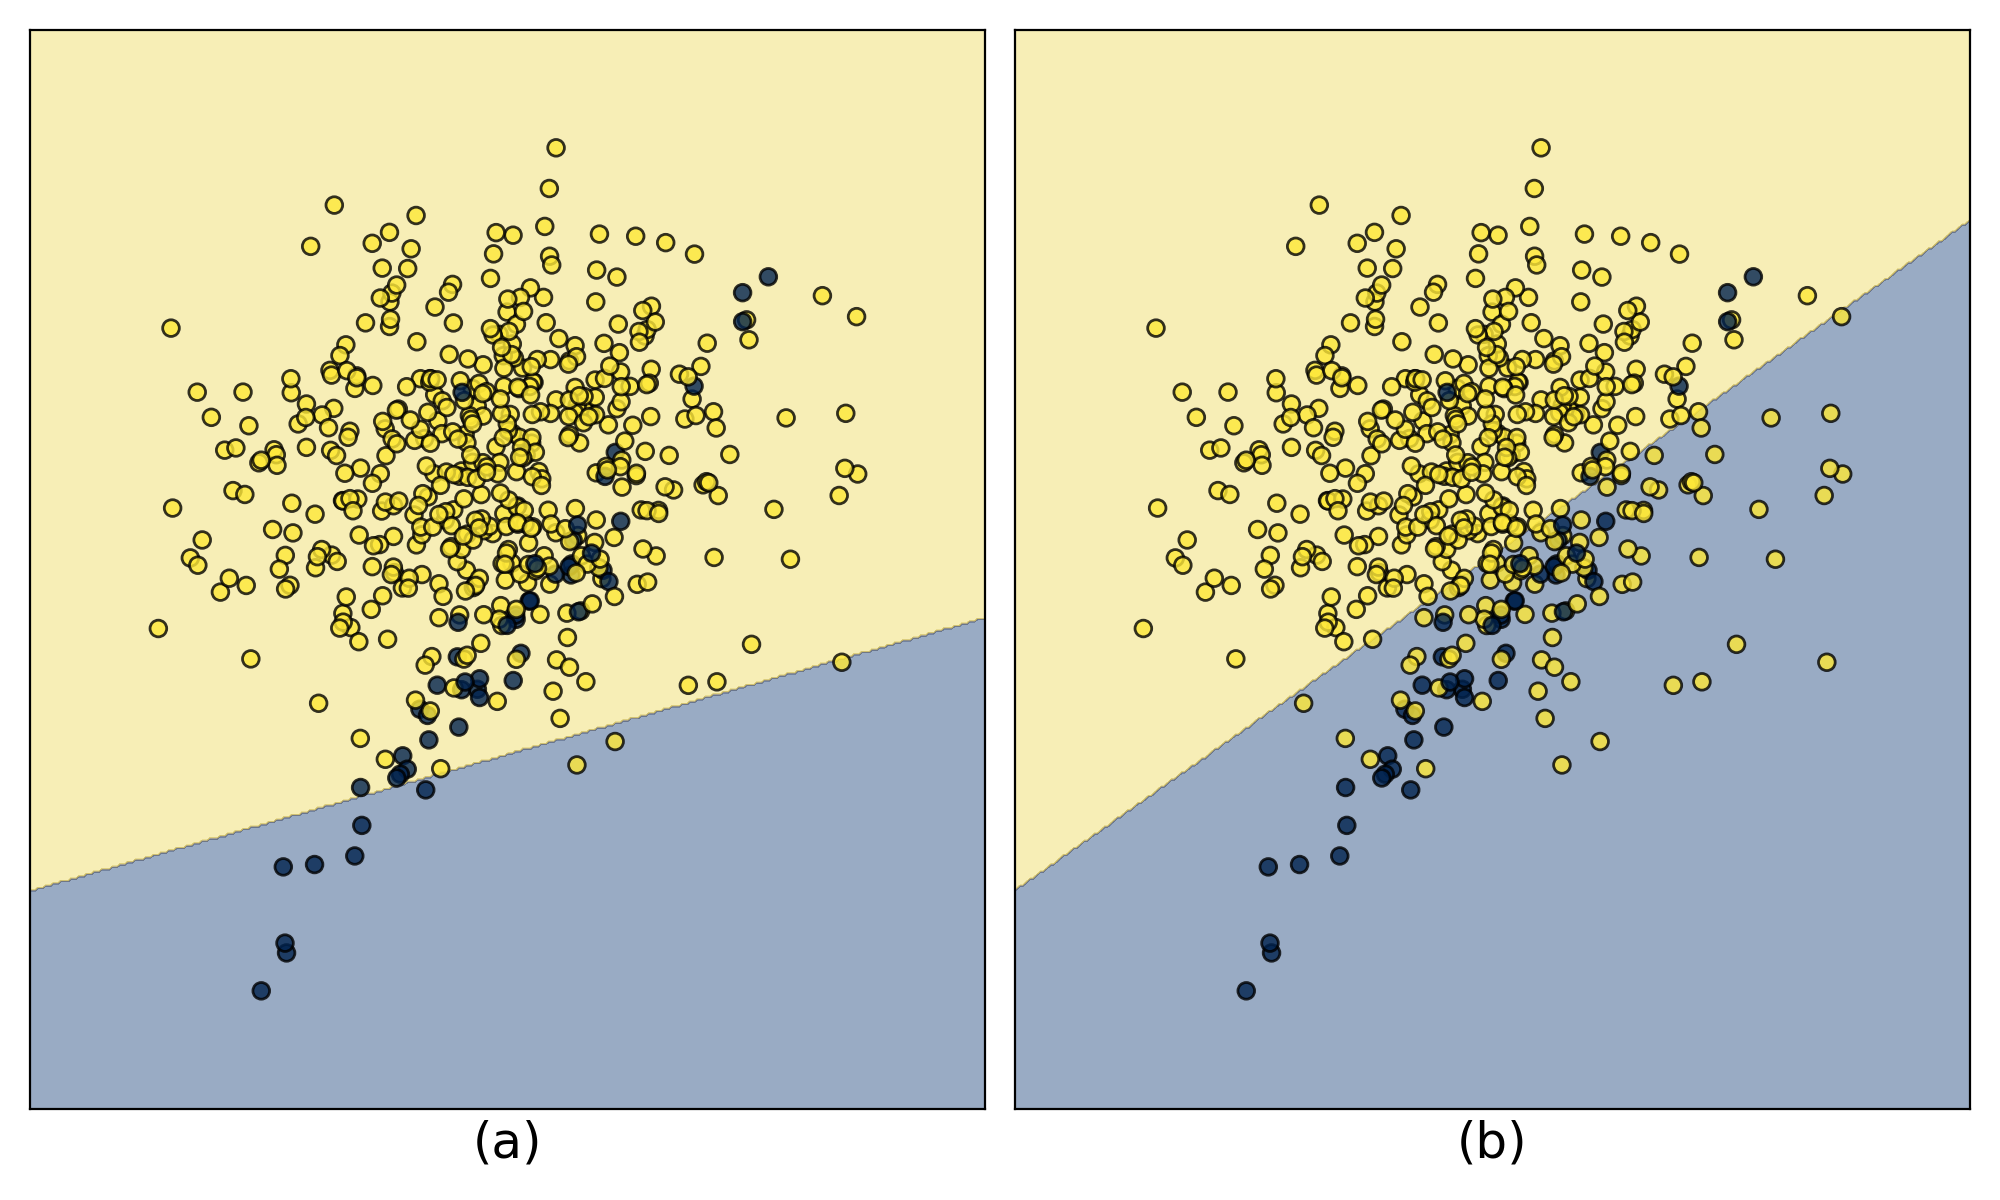
\includegraphics[width=.75\linewidth]{../analysis/oversampling_decision_function}
	\caption{Example of a linear Support Vector Machine's decision function (a) without
		resampling and (b) with resampling.}
	\label{fig:oversampling_decision_function}
\end{figure}

In this paper, we propose the K-means SMOTE (K-SMOTE) \cite{Douzas2018}
oversampler to address the imbalanced learning problem in a multiclass context
for LULC classification in various reference remote sensing datasets. K-SMOTE's
efficacy is tested using different types of classifiers. To do so, we employ
both commonly used and state-of-the-art oversamplers as benchmarking methods:
Random oversampling (ROS), Synthetic Minority Oversampling Technique (SMOTE)
\cite{Chawla2002} and Borderline-SMOTE (B-SMOTE) \cite{Han2005}.
As a baseline we present classification results without the employment of any
resampling method.

This paper is organized in 5 sections: section \ref{sec:sota} provides
an overview of the state-of-art, section \ref{sec:methodology} describes the
proposed methodology, section \ref{sec:results} covers the results and
discussion and section \ref{sec:conclusion} presents the conclusions taken
from this study.

\section{Imbalanced Learning Approaches} \label{sec:sota}

Existing methods that address imbalanced learning act on different stages. They
can act in the preprocessing step (Over/Undersampling and hybrid approaches),
in the learning process (cost-sensitive solutions) or in the algorithm itself
(by adapting existing algorithms and/or ensemble methods)
\cite{Kaur2019}. In this section, we focus on previous work related
with resampling methods, while providing a brief explanation of cost-sensitive
and algorithmic level solutions.

All of the most common classifiers used for LULC classification tasks
\cite{Khatami2016, Gavade2019} are sensitive to class imbalance
\cite{Blagus2010}. Algorithm-based approaches typically focus on
adaptations based on ensemble classification methods \cite{Mellor2015} or
common non-ensemble based classifiers such as Support Vector Machines
\cite{Shao2014}. In \cite{Lee2016}, the reported results show
that algorithm-based methods have comparable performance to resampling methods.

Cost-sensitive solutions refer to changes in the importance attributed to each
instance through a cost matrix \cite{Huang2016,Cui2019,Dong2017}. A common cost sensitive
solution is found in \cite{Huang2016}. The authors use the inverse class
frequency (i.e., $1/|C_i|$) to give higher weight to minority
classes. Cui et al. \cite{Cui2019} extended this method by adding a
hyperparameter $\beta$ to class weights as
$(1-\beta)/(1-\beta^{|C_i|})$. When $\beta=0$, no re-weighting is done.
When $\beta\rightarrow 1$, weights are the inverse of the frequency class
matrix. Another method \cite{Dong2017} explores adaptations of
Cross-entropy classification loss by adding different formulations of class
rectification loss.

Imbalanced Learning is most commonly addressed through data resampling in
machine learning in general and remote sensing in particular
\cite{Feng2019}. The generation of artificial instances (i.e.,
augmenting the dataset) based on rare examples is done independently of any
other classification and preprocessing step. Once this step is applied, any
standard ML procedure can be applied. This simplicity makes resampling
strategies particularly appealing for any user interested in applying several
classifiers or maintaining a simple approach. Additionally, any of these
methods can be naturally applied to multiclass problems and particularly to
LULC classification tasks.

\subsection{Non-informed resampling methods}

There are two main non-informed resampling methods. Random Oversampling (ROS)
generates artificial observations through random duplication of rare instances.
This method is used in remote sensing \cite{Sharififar2019, Hounkpatin2018} for its
simplicity, even though its mechanism makes the classifier prone to overfitting
\cite{Krawczyk2016}. Hounkpatin et al. \cite{Hounkpatin2018} found that
using ROS returned worse results than keeping the original imbalance in their
dataset.

A few of the recent remote sensing studies employed Random Undersampling (RUS)
\cite{Ferreira2019}. This method, on the other hand, randomly removes
observations belonging to common classes. Although it's not as prone to
overfitting as ROS, it incurs into information loss by eliminating observations
from the majority class \cite{Feng2019}.

Another downfall of non-informed resampling methods is their performance-wise
inconsistency across classifiers. ROS' impact on the Indian Pines dataset was
found inconsistent between Random Forest Classifiers (RFC) and Support Vector
Machines (SVM) and lowered the predictive power of an artificial neural network
(ANN) \cite{Maxwell2018}. Similarly, RUS is found to generally lead to a
lower overall accuracy due to the associated information loss
\cite{Maxwell2018}.

\subsection{Heuristic methods}

The methods presented in this section appear as a means to overcome the
insufficiencies found in non-informed resampling. They use either local or
global information to generate new, relevant, non-duplicated instances to
populate the minority classes and/or remove irrelevant instances from majority
classes. In a comparative analysis between over- and undersamplers' performance
for LULC classification \cite{Feng2018} using the rotation forest
ensemble classifier, authors found that oversampling methods consistently
outperform undersampling methods. Due to the scope of this study, heuristic
undersampling algorithms will not be analysed.

SMOTE \cite{Chawla2002} was the first heuristic oversampling algorithm to
be proposed and has been the most popular one since then, likely due to its
fair degree of simplicity and quality of generated data. It takes a random
minority class sample and introduces synthetic examples along the line segments
that join any/all of the $k$ minority class nearest
neighbors to the selected sample. Specifically, a single synthetic sample
$\overrightarrow{z}$ is generated within the line segment of a randomly
selected minority class observation $\overrightarrow{x}$ and one of its
$k$ nearest neighbors $\overrightarrow{y}$ such that
$\overrightarrow{z} =
	\alpha\overrightarrow{x}+(1-\alpha)\overrightarrow{y}$, where $\alpha$ is a random floating point
between 0 and 1, as shown in Figure \ref{fig:smote_example}.

\begin{figure}[H]
	\centering
	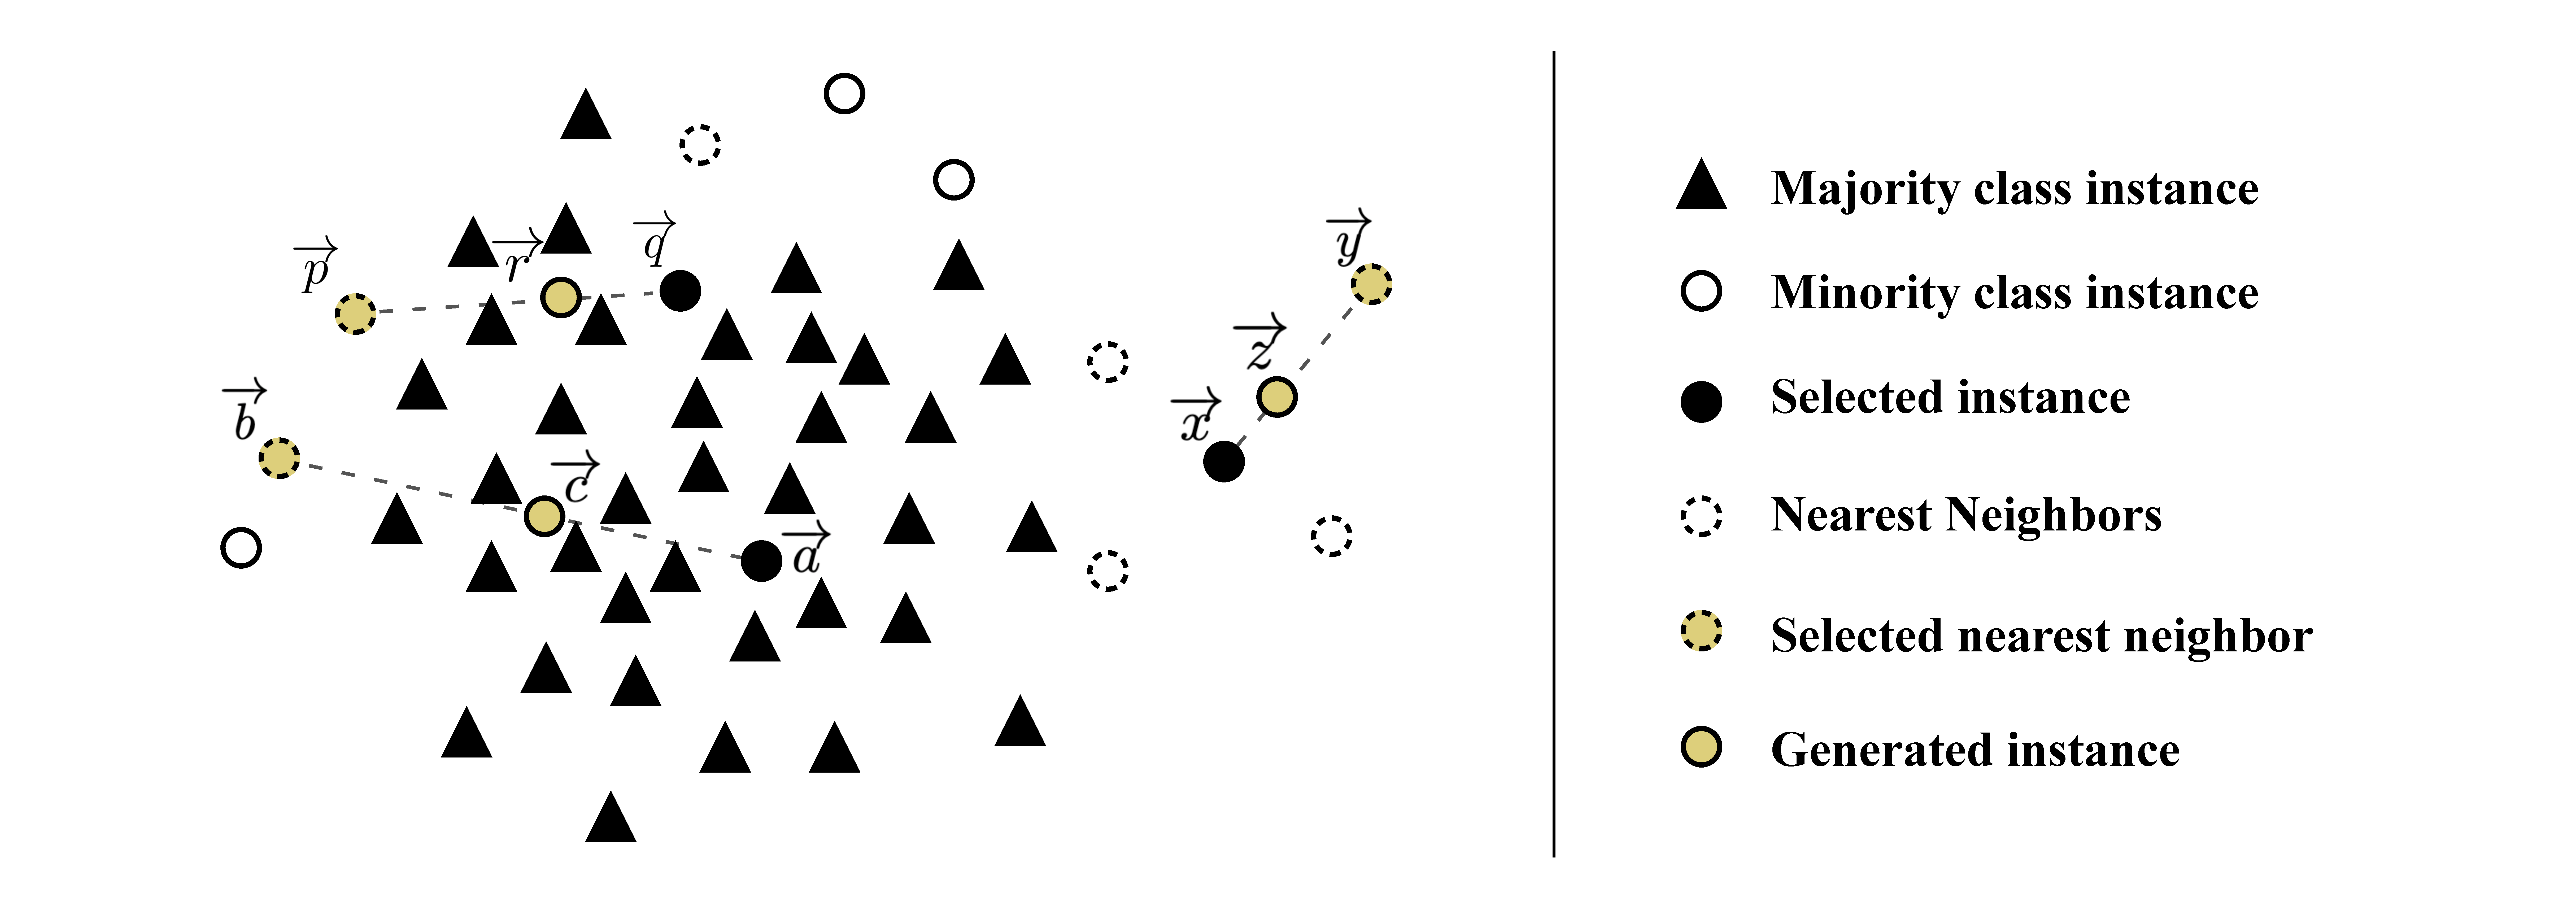
\includegraphics[width=1\linewidth]{../analysis/smote_example}
	\caption{Example of SMOTE's data generation process.}
	\label{fig:smote_example}
\end{figure}

A number of studies implement SMOTE within the LULC classification context and
reported improvements on the quality of the trained predictors
\cite{Jozdani2019, Bogner2018}. Another study proposes an adaptation of SMOTE on an
algorithmic level for deep learning applications \cite{Zhu2020}. This
method combines both typical computer vision data augmentation techniques, such
as image rotation, scaling and flipping on the generated instances to populate
minority classes. Another algorithmic implementation is the variational
semi-supervised learning model \cite{Cenggoro2018}. It consists of a
generative model that allows learning from both labelled and unlabelled
instances while using SMOTE to balance the data.

Despite SMOTE's popularity, its drawbacks motivated the development of more
sophisticated oversampling algorithms \cite{Douzas2019}:
\begin{enumerate}
	\item Generation of noisy instances due to random selection of a minority observation
	      to oversample. The random selection of a minority observation makes SMOTE
	      oversampling prone to the amplification of existing noisy data. In Figure
	      \ref{fig:smote_example} it is possible to observe a minority sample located
	      within a cluster of majority instances. Performing a linear interpolation
	      between the noisy sample $\overrightarrow{a}$ and one of its nearest neighbors
	      $\overrightarrow{b}$ will generate a noisy sample $\overrightarrow{c}$.
	      B-SMOTE \cite{Han2005} attempts to circumvent the noisy data selection
	      problem by performing a targeted selection of instances close to the presumed
	      class border, determined by the labels of each sample's $k$
	      nearest neighbors. Alternatively, a sample will discarded because it was deemed
	      as either noisy, or being far from the class boundary. Another algorithm that
	      addresses this problem is ADASYN \cite{HaiboHe2008}. It calculates a
	      density distribution ratio for each sample based on its
	      $k$-nearest neighbors to determine the number of synthetic
	      observations to generate for each minority class observation using the
	      described SMOTE procedure.

	\item Generation of noisy instances due to the selection of the $k$
	      nearest neighbors. In the event an observation (or a small number thereof) is
	      not noisy but is isolated from the remaining clusters, known as the "small
	      disjuncts problem" \cite{holte1989}, much like sample
	      $\overrightarrow{b}$ from Figure \ref{fig:smote_example}, the selection of any
	      nearest neighbor of the same class will have a high likelihood of producing a
	      noisy sample.

	\item Generation of nearly duplicated instances. Whenever the linear interpolation is
	      done between two observations that are close to each other, the generated
	      instance becomes very similar to its parents and increases the risk of
	      overfitting. G-SMOTE \cite{Douzas2019} attempts to address both the
	      $k$ nearest neighbor selection mechanism problem as well as
	      the generation of nearly duplicated instances problem. It proposes a variation
	      on SMOTE's data generation mechanism by generating data within an oval geometry
	      (instead of a line segment) around the selected observation and the selected
	      nearest neighbor. In its turn, the $k$ nearest neighbors
	      selection can include observations from the remaining classes. To an extent,
	      this algorithm can be considered a generalized version of SMOTE, since under
	      specific hyperparameter definitions it replicates SMOTE's behavior.

	\item Generation of noisy instances due to the use of observations from two different
	      minority class clusters. Although an increased $k$ could
	      potentially avoid the previous problem, it can also lead to the generation of
	      artificial data between different minority clusters. Cluster-based oversampling
	      methods, as well as ADASYN, attempt to address this problem. B-SMOTE
	      \cite{Han2005} and G-SMOTE also address this problem by allowing the
	      interpolation to be performed with majority class instances.
\end{enumerate}

Although no cluster-based oversampling approach applied within the remote
sensing domain was found in the literature, there are numerous methods to
consider. Cluster-based oversampling approaches introduce an additional layer
to SMOTE's selection mechanism, which is done according to the clustering
process. This is done to ensure both between-class data balance, but also
ensure that the data distribution within each class is preserved. The
self-organizing map oversampling (SOMO) \cite{Douzas2017} algorithm
transforms the dataset into a 2-dimensional input, where the areas with the
highest density of minority samples are identified. SMOTE is then used to
oversample each of the identified areas separately. CURE-SMOTE
\cite{Ma2017} applies a hierarchical clustering algorithm (CURE) to
discard isolated minority instances before applying SMOTE. Although it avoids
noise generation problems, it ignores within-class data distribution. Another
method \cite{Santos2015} uses K-means to cluster the entire input space
and applies SMOTE to clusters the the fewest representations, regardless of the
observations' class label. The label of the generated observation is copied
from one of its parents. This method cannot ensure a balanced dataset, class
imbalance is not specifically addressed, but rather dataset imbalance.

K-SMOTE \cite{Douzas2018} avoids noisy data generation by modifying the
data selection mechanism. It employs $k$-means clustering to
identify safe areas using cluster-specific Imbalance Ratio (defined by
$\frac{count(C_{majority})}{count(C_{minority})}$) and determine the quantity of generated samples per
cluster based on a density measure. These samples are finally generated using
the SMOTE algorithm. The K-SMOTE's data generation process is depicted in
Figure \ref{fig:kmeans_smote_example}. Note that the number of samples generated for
each cluster varies according to the sparsity of each cluster (the sparser the
cluster is, the more samples will be generated) and a cluster is rejected if
the cluster's IR surpasses the threshold. Therefore, this method can be
combined with oversamplers focused on data generation, such as G-SMOTE.

\begin{figure}[H]
	\centering
	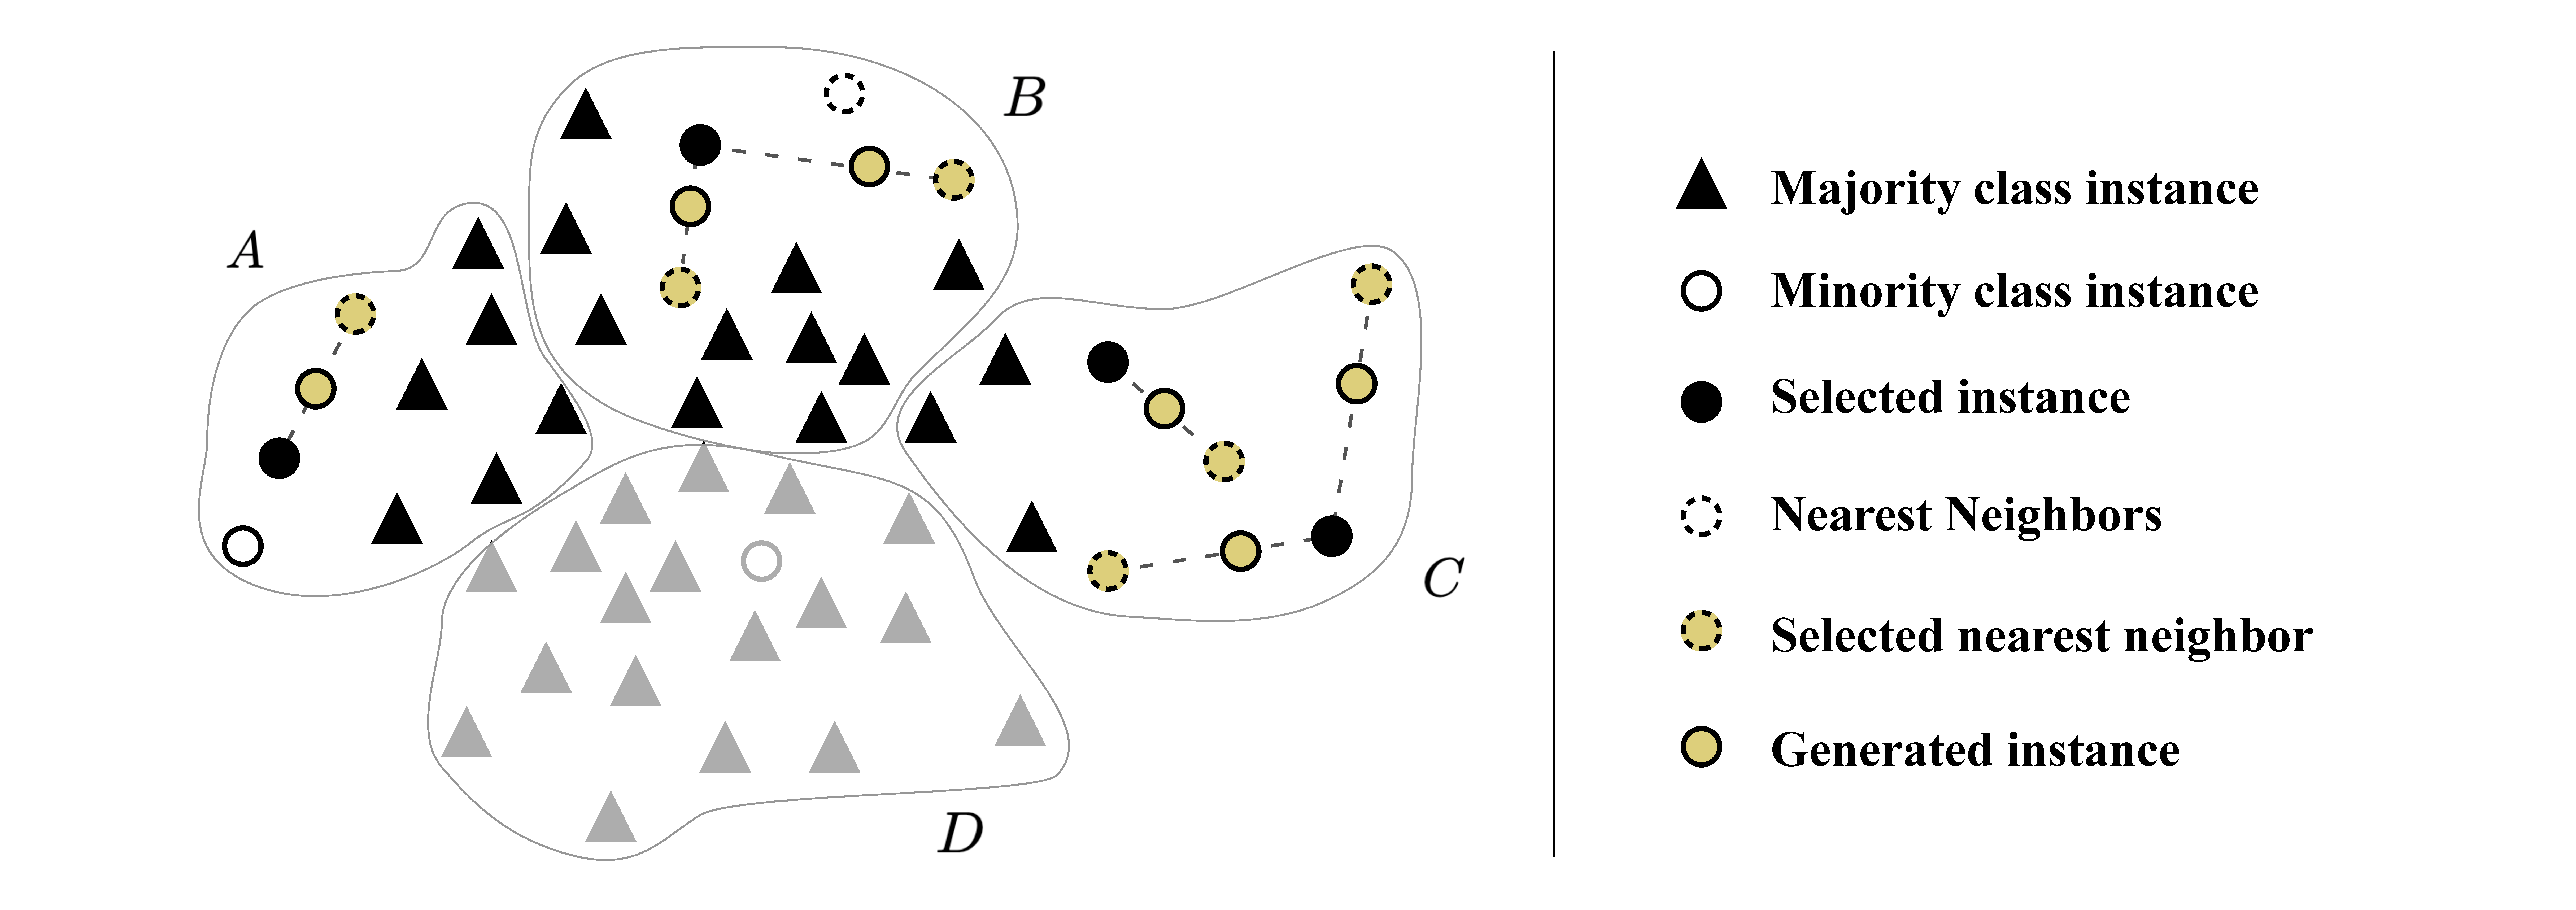
\includegraphics[width=1\linewidth]{../analysis/kmeans_smote_example}
	\caption{Example of K-SMOTE's data generation process. Clusters $A$,
		$B$ and $C$ are selected for
		oversampling, whereas cluster $D$ was rejected due to its
		high imbalance ratio. The oversampling is done using the SMOTE algorithm and
		the $k$ nearest neighbors selection only considers
		observations within the same cluster.}
	\label{fig:kmeans_smote_example}
\end{figure}

Although no other study was found to implement cluster-based oversampling,
another study \cite{Douzas2019rs} compared the performance of SMOTE, ROS,
ADASYN, B-SMOTE and G-SMOTE in a highly imbalanced LULC classification dataset.
The authors found that G-SMOTE consistently outperformed the remaining
oversampling algorithms regardless of the classifier used.

This paper main contributions are:
\begin{itemize}
	\item Testing these oversampling methods in multiple widely used LULC classification
	      datasets. Allows us to check for oversamplers' performance statistical
	      significance across datasets and report K-SMOTE's performance in benchmark LULC
	      datasets.
	\item Introducing a cluster-based oversampling algorithm within the remote sensing
	      domain, as well as comparing its performance with the remaining oversamplers in
	      a multiclass context.

\end{itemize}

\section{Methodology} \label{sec:methodology}

The purpose of this work is to understand the performance of K-SMOTE as opposed
to other popular and/or state-of-the-art oversamplers for LULC classification.
To do so, we employ 7 LULC datasets along with 3 evaluation metrics and 5
classifiers to evaluate the performance of oversamplers. In this section we
describe the datasets, evaluation metrics, oversamplers, classifiers and
software used as well as the procedure developed.

\subsection{Datasets}

The datasets used were extracted from publicly available hyperspectral scenes.
Information regarding each of these scenes is provided in this subsection. A
similar data preprocessing procedure was used for each scene: 1) Conversion of
hyperspectral scene to structured dataset, 2) removal of instances with no
associated LULC class and 3) stratified random sampling. The last step is done
in order to downsample the datasets to a practicable size due to computational
constraints (2000 instances per dataset), while conserving the relative LULC
class frequencies and data distribution. Table \ref{tab:datasets_description} provides
a description of the final datasets used for this work.

\pgfplotstabletypeset[
	begin table=\begin{longtable},
		end table=\end{longtable},  col sep=comma, header=true,
	columns={Dataset,Features,Instances,Minority instances,Majority instances,IR, Classes}, string type, every head row/.style={before row=\toprule, after row=\midrule\endhead},
	every last row/.style={after row=\bottomrule \caption{\label{tab:datasets_description}
				Description of the datasets used for this experiment.}}
]{../analysis/datasets_description.csv}

\subsubsection*{Indian Pines}
The Indian Pines scene \cite{Baumgardner2015} was collected on June 12, 1992
and consists of AVIRIS hyperspectral image data covering the Indian Pine Test
Site 3, located in North-western Indiana, USA. As a subset of a larger scene,
it is composed of $145 \times 145$ pixels (see Figure
\ref{fig:indian_pines}) and 220 spectral reflectance bands in the wavelength
range 400 to 2500 nanometers. Approximately two thirds of this scene is
composed by agriculture and the other third is composed of forest and other
natural perennial vegetation. Additionally, the scene also contains low density
buildup areas.

\subsubsection*{Pavia Centre and University}
Both Pavia Centre and University scenes were acquired by the ROSIS sensor.
These scenes are located in Pavia, northern Italy. Pavia Centre is a
$1096 \times 1096$ pixels image with 102 spectral bands, whereas Pavia
University is a $610 \times 610$ pixels image with 103 spectral bands.
Both images have a geometrical resolution of 1.3 meters and their ground truths
are composed of 9 classes each (see Figures \ref{fig:pavia_centre} and
\ref{fig:pavia_university}).

\subsubsection*{Salinas and Salinas-A}
These scenes were collected by the AVIRIS sensor over Salinas Valley,
California and contain at-sensor radiance data. Salinas is a
$512 \times 217$ pixels image with 224 bands and 16 classes regarding
vegetables, bare soil and vineyard fields (see Figure \ref{fig:salinas}).
Salinas-A, a subscene of Salinas, comprises $86 \times 83$ pixels and
contains 6 classes regarding vegetables (see Figure \ref{fig:salinas_a}).
These scenes have a geometrical resolution of 3.7 meters.

\subsubsection*{Botswana}
The Botswana scene was acquired by the Hyperion sensor on the NASA EO-1
satellite over the Okavango Delta, Botswana in 2001-2004 at a 30m spatial
resolution. Data preprocessing was performed by the UT Center for Space
Research. The scene comprises a $1476 \times 256$ pixels with 145 bands
and 14 classes regarding land cover types in seasonal and occasional swamps, as
well as drier woodlands (see figure \ref{fig:botswana}).

\subsubsection*{Kennedy Space Center}
The Kennedy Space Center scene was acquired by the AVIRIS sensor over the
Kennedy Space Center, Florida, on March 23, 1996. Out of the original 224
bands, water absorption and low SNR bands were removed and a total of 176 bands
at a spatial resolution of 18m are used. The scene is a $512 \times 614$
pixel image and contains a total of 16 classes (see figure
\ref{fig:kennedy_space_center}).

\begin{figure}[H]
	\centering
	\begin{subfigure}{.24\textwidth}
		\centering
		\captionsetup{skip=12pt}
		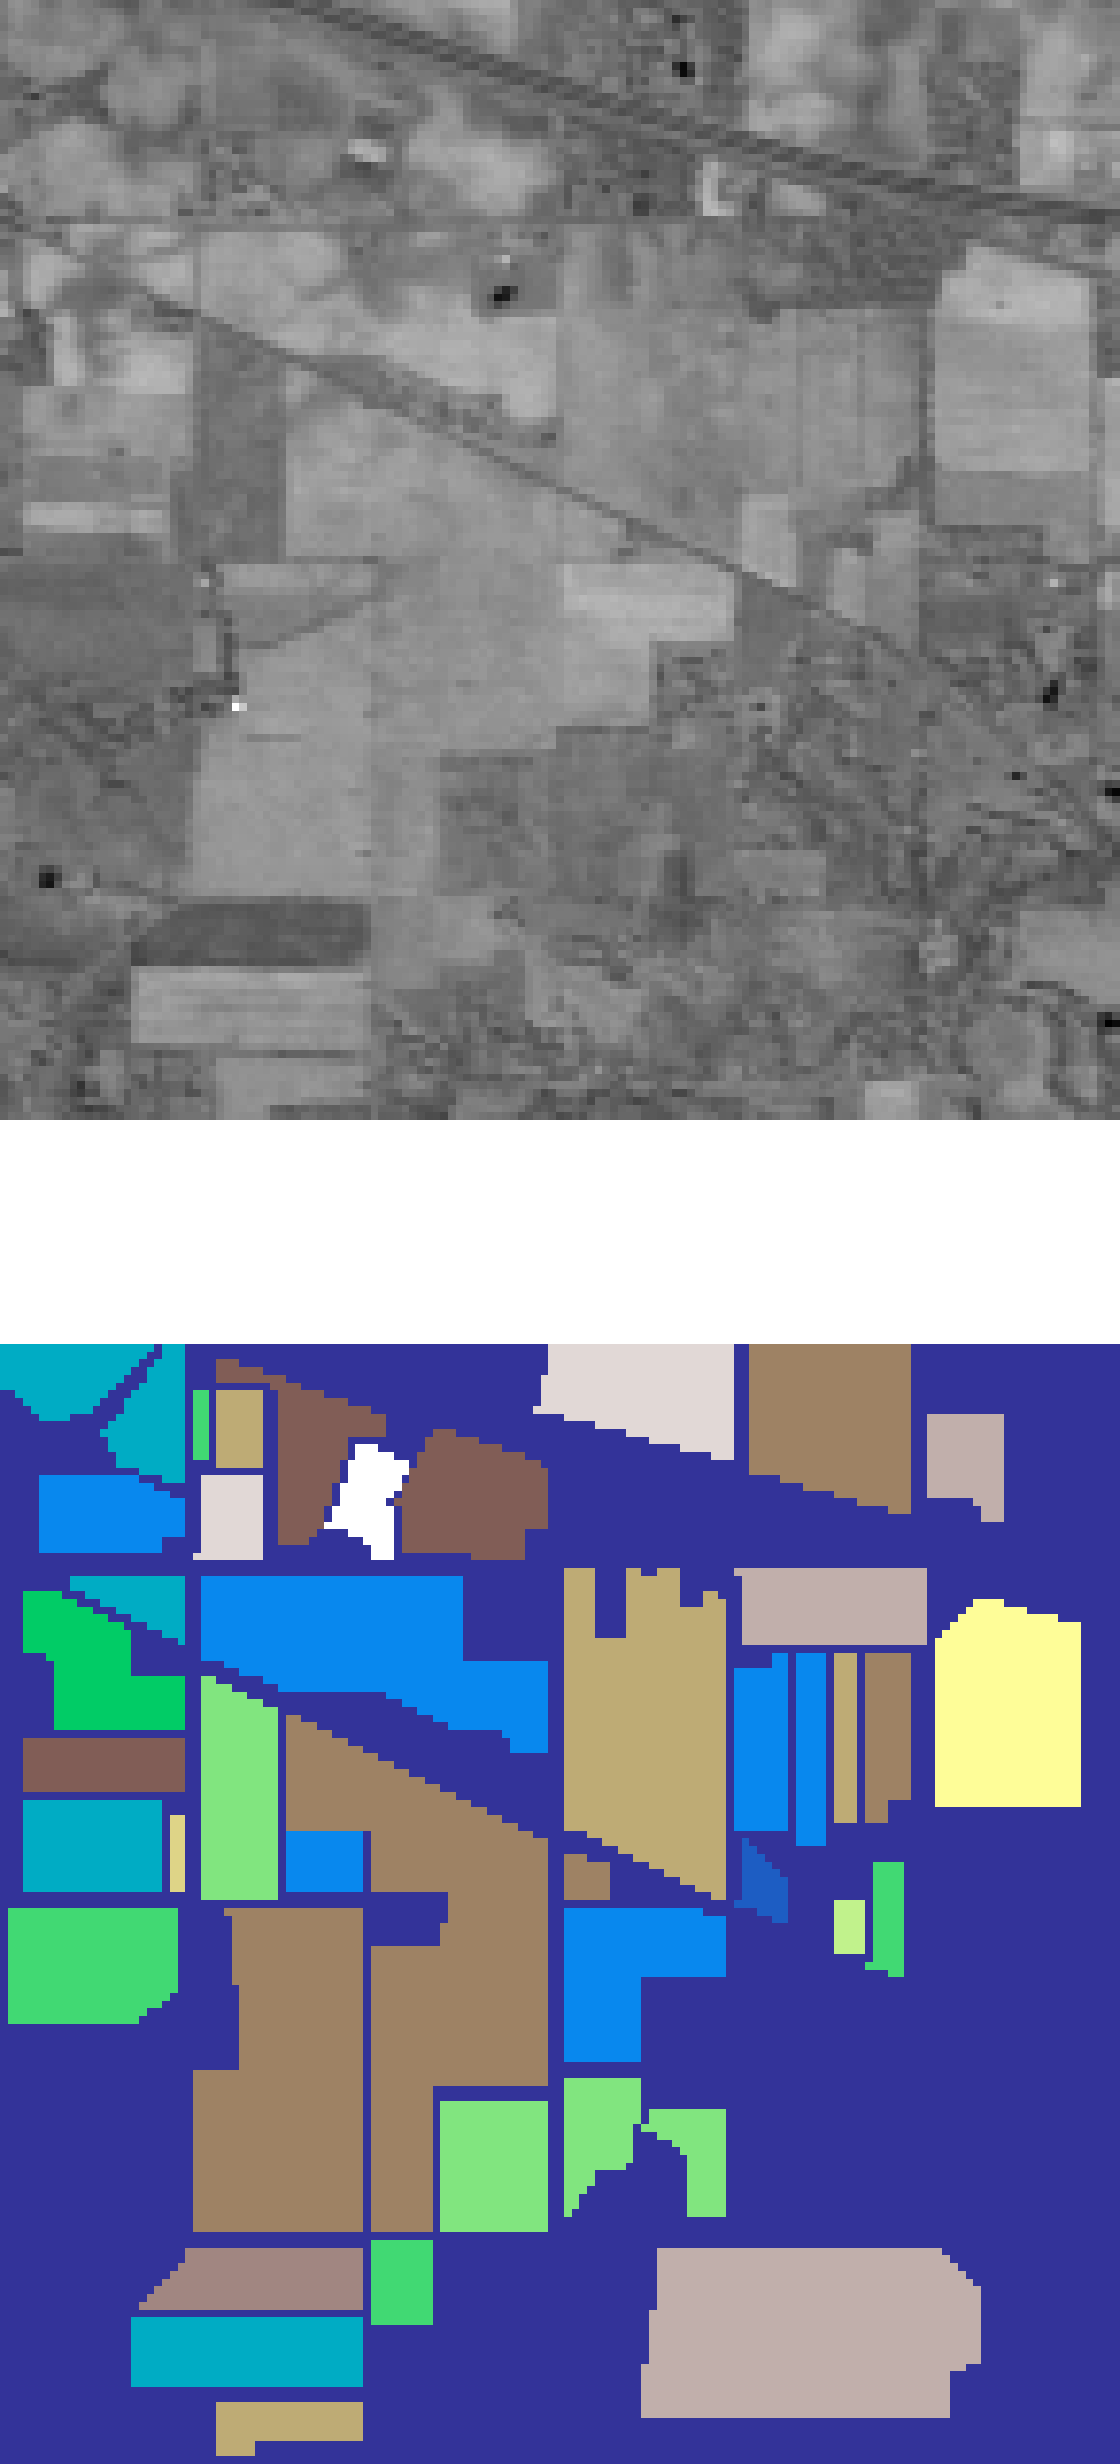
\includegraphics[height=1.9\linewidth]{../analysis/indian_pines}
		\subcaption{{\medbreak}}
		\label{fig:indian_pines}
	\end{subfigure}
	\begin{subfigure}{.24\textwidth}
		\centering
		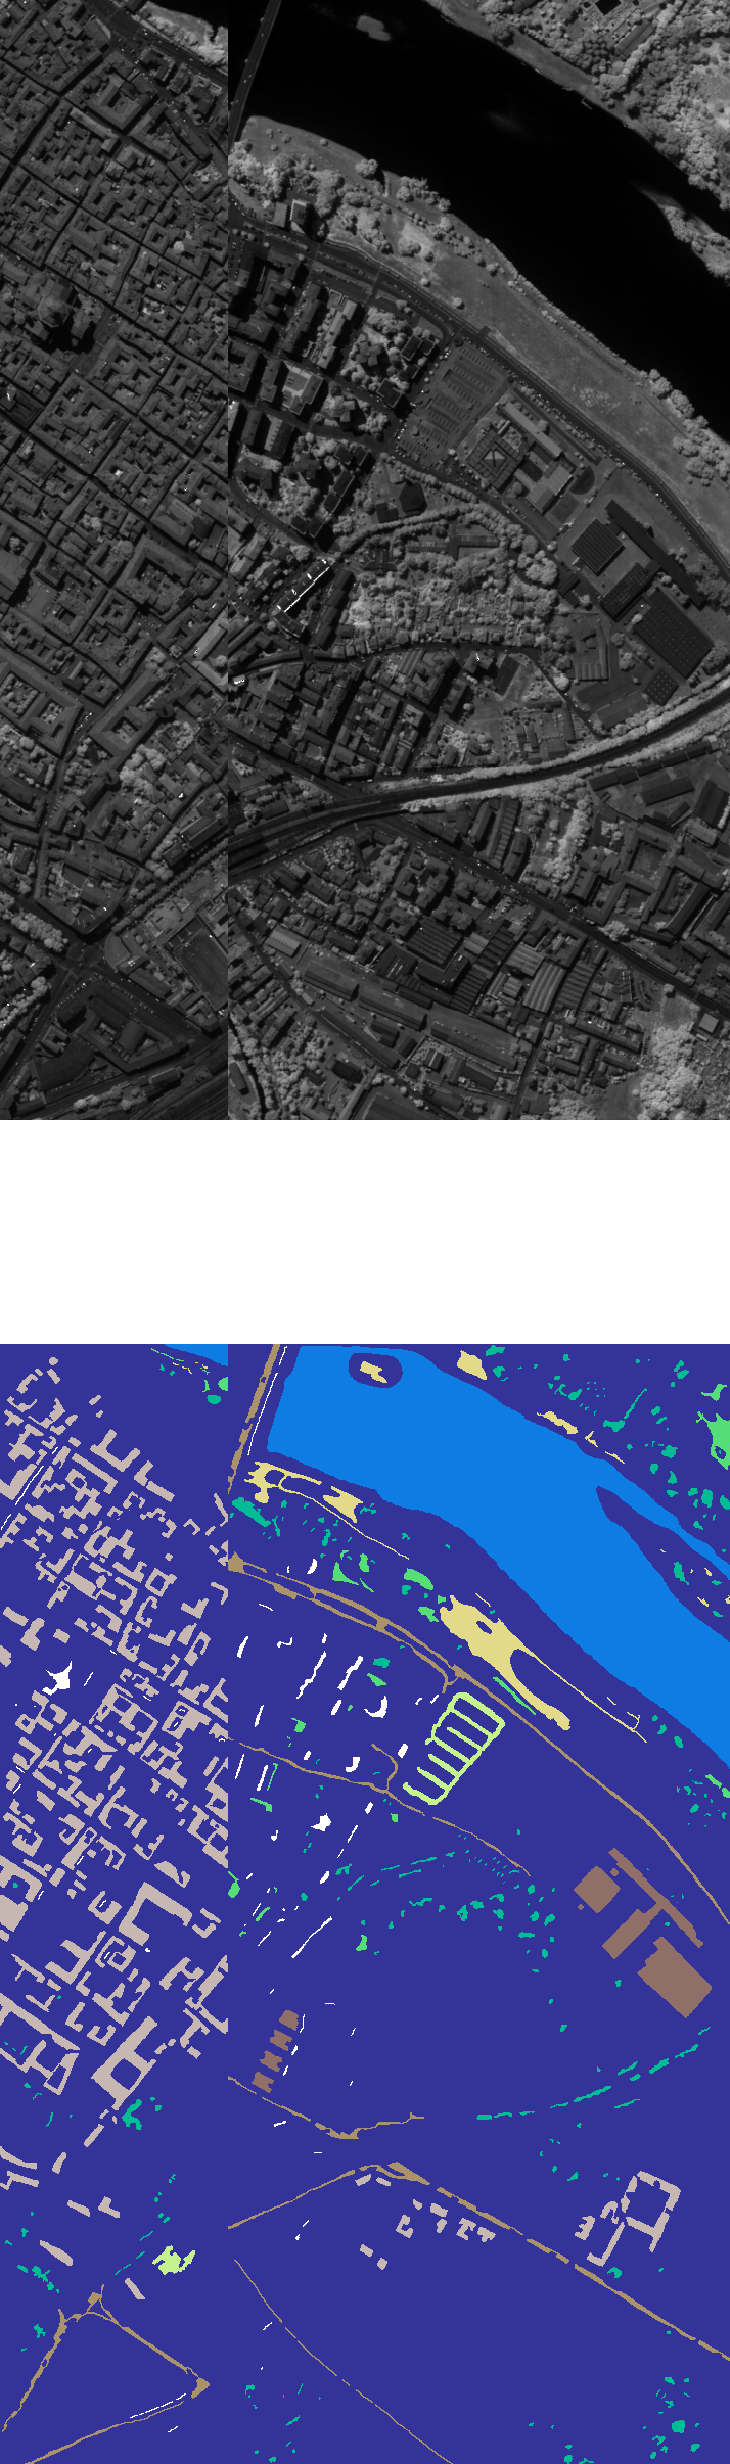
\includegraphics[height=1.9\linewidth]{../analysis/pavia_centre}
		\subcaption{{\medbreak}}
		\label{fig:pavia_centre}
	\end{subfigure}
	\begin{subfigure}{.24\textwidth}
		\centering
		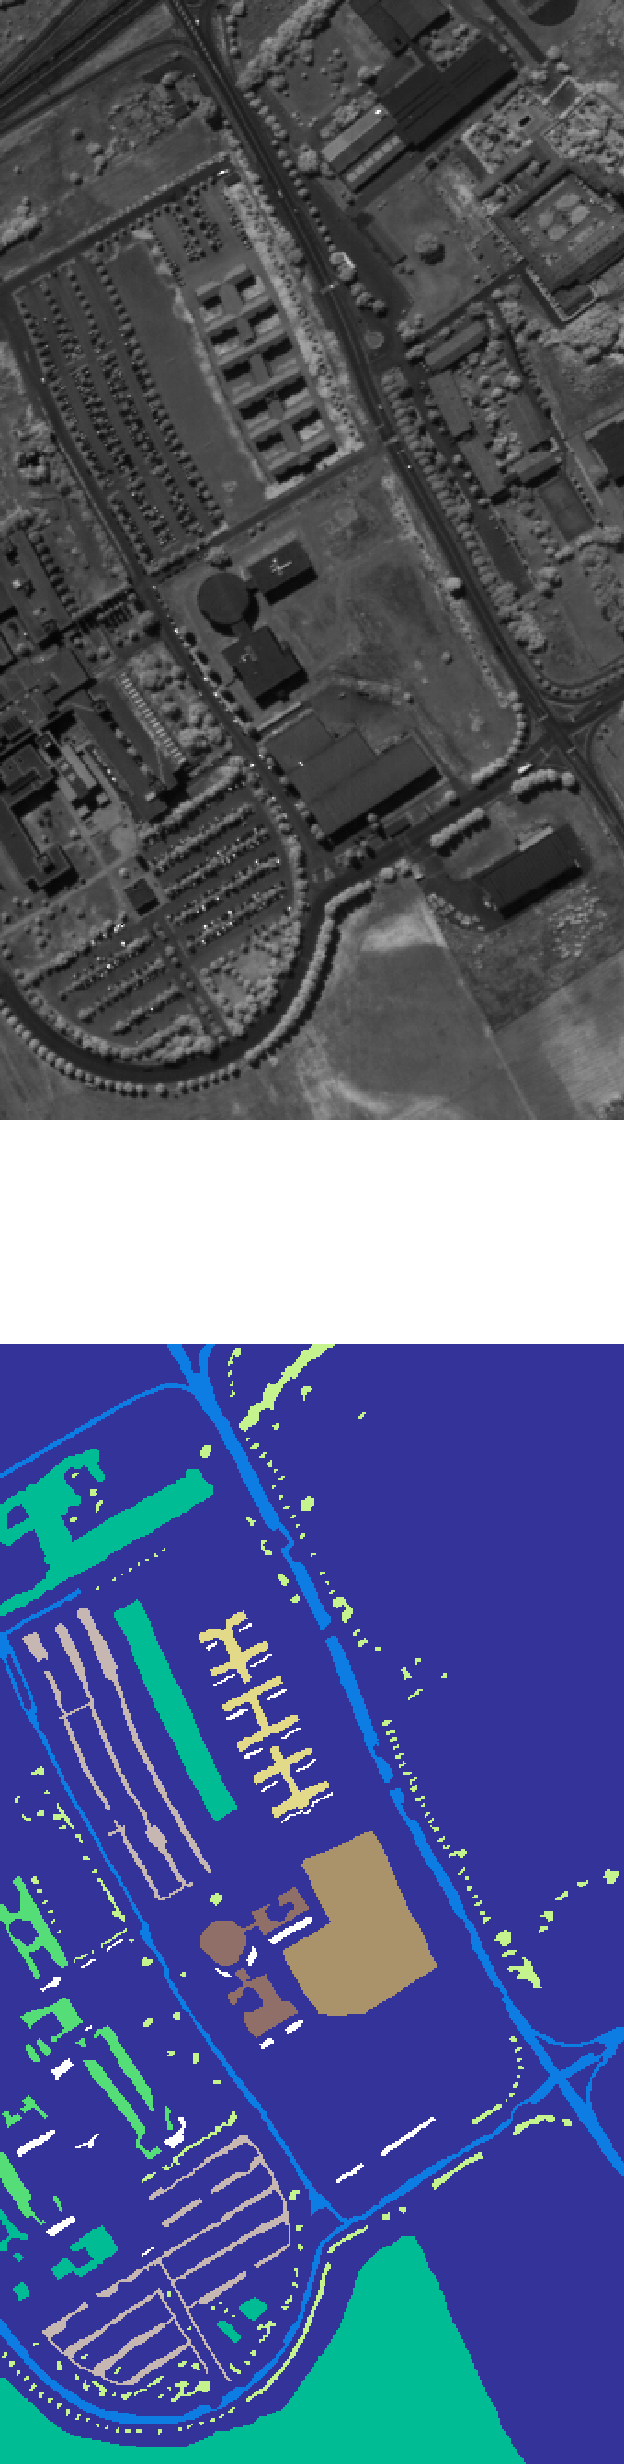
\includegraphics[height=1.9\linewidth]{../analysis/pavia_university}
		\subcaption{{\medbreak}}
		\label{fig:pavia_university}
	\end{subfigure}

	\begin{subfigure}{.24\textwidth}
		\centering
		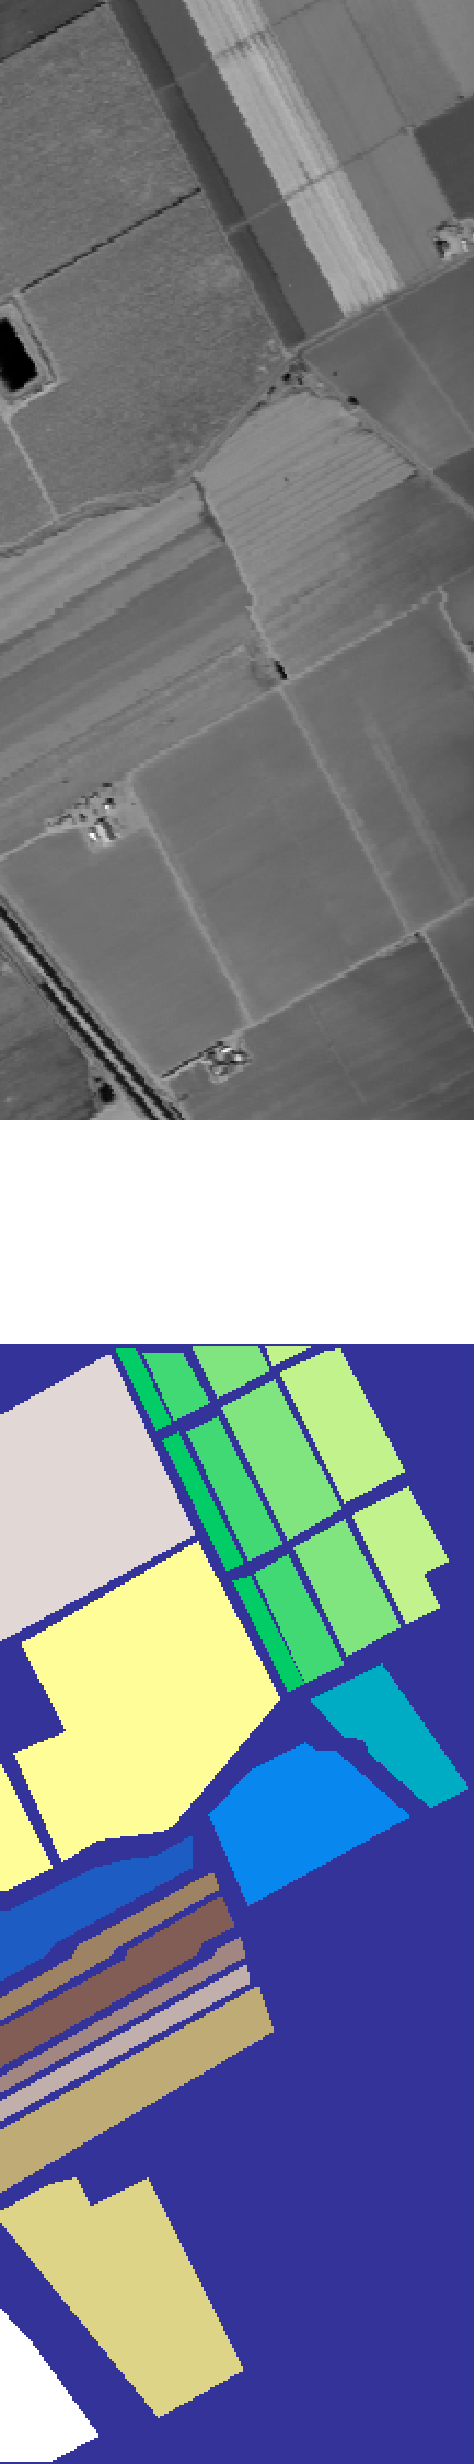
\includegraphics[height=1.9\linewidth]{../analysis/salinas}
		\subcaption{{\medbreak}}
		\label{fig:salinas}
	\end{subfigure}
	\begin{subfigure}{.24\textwidth}
		\centering
		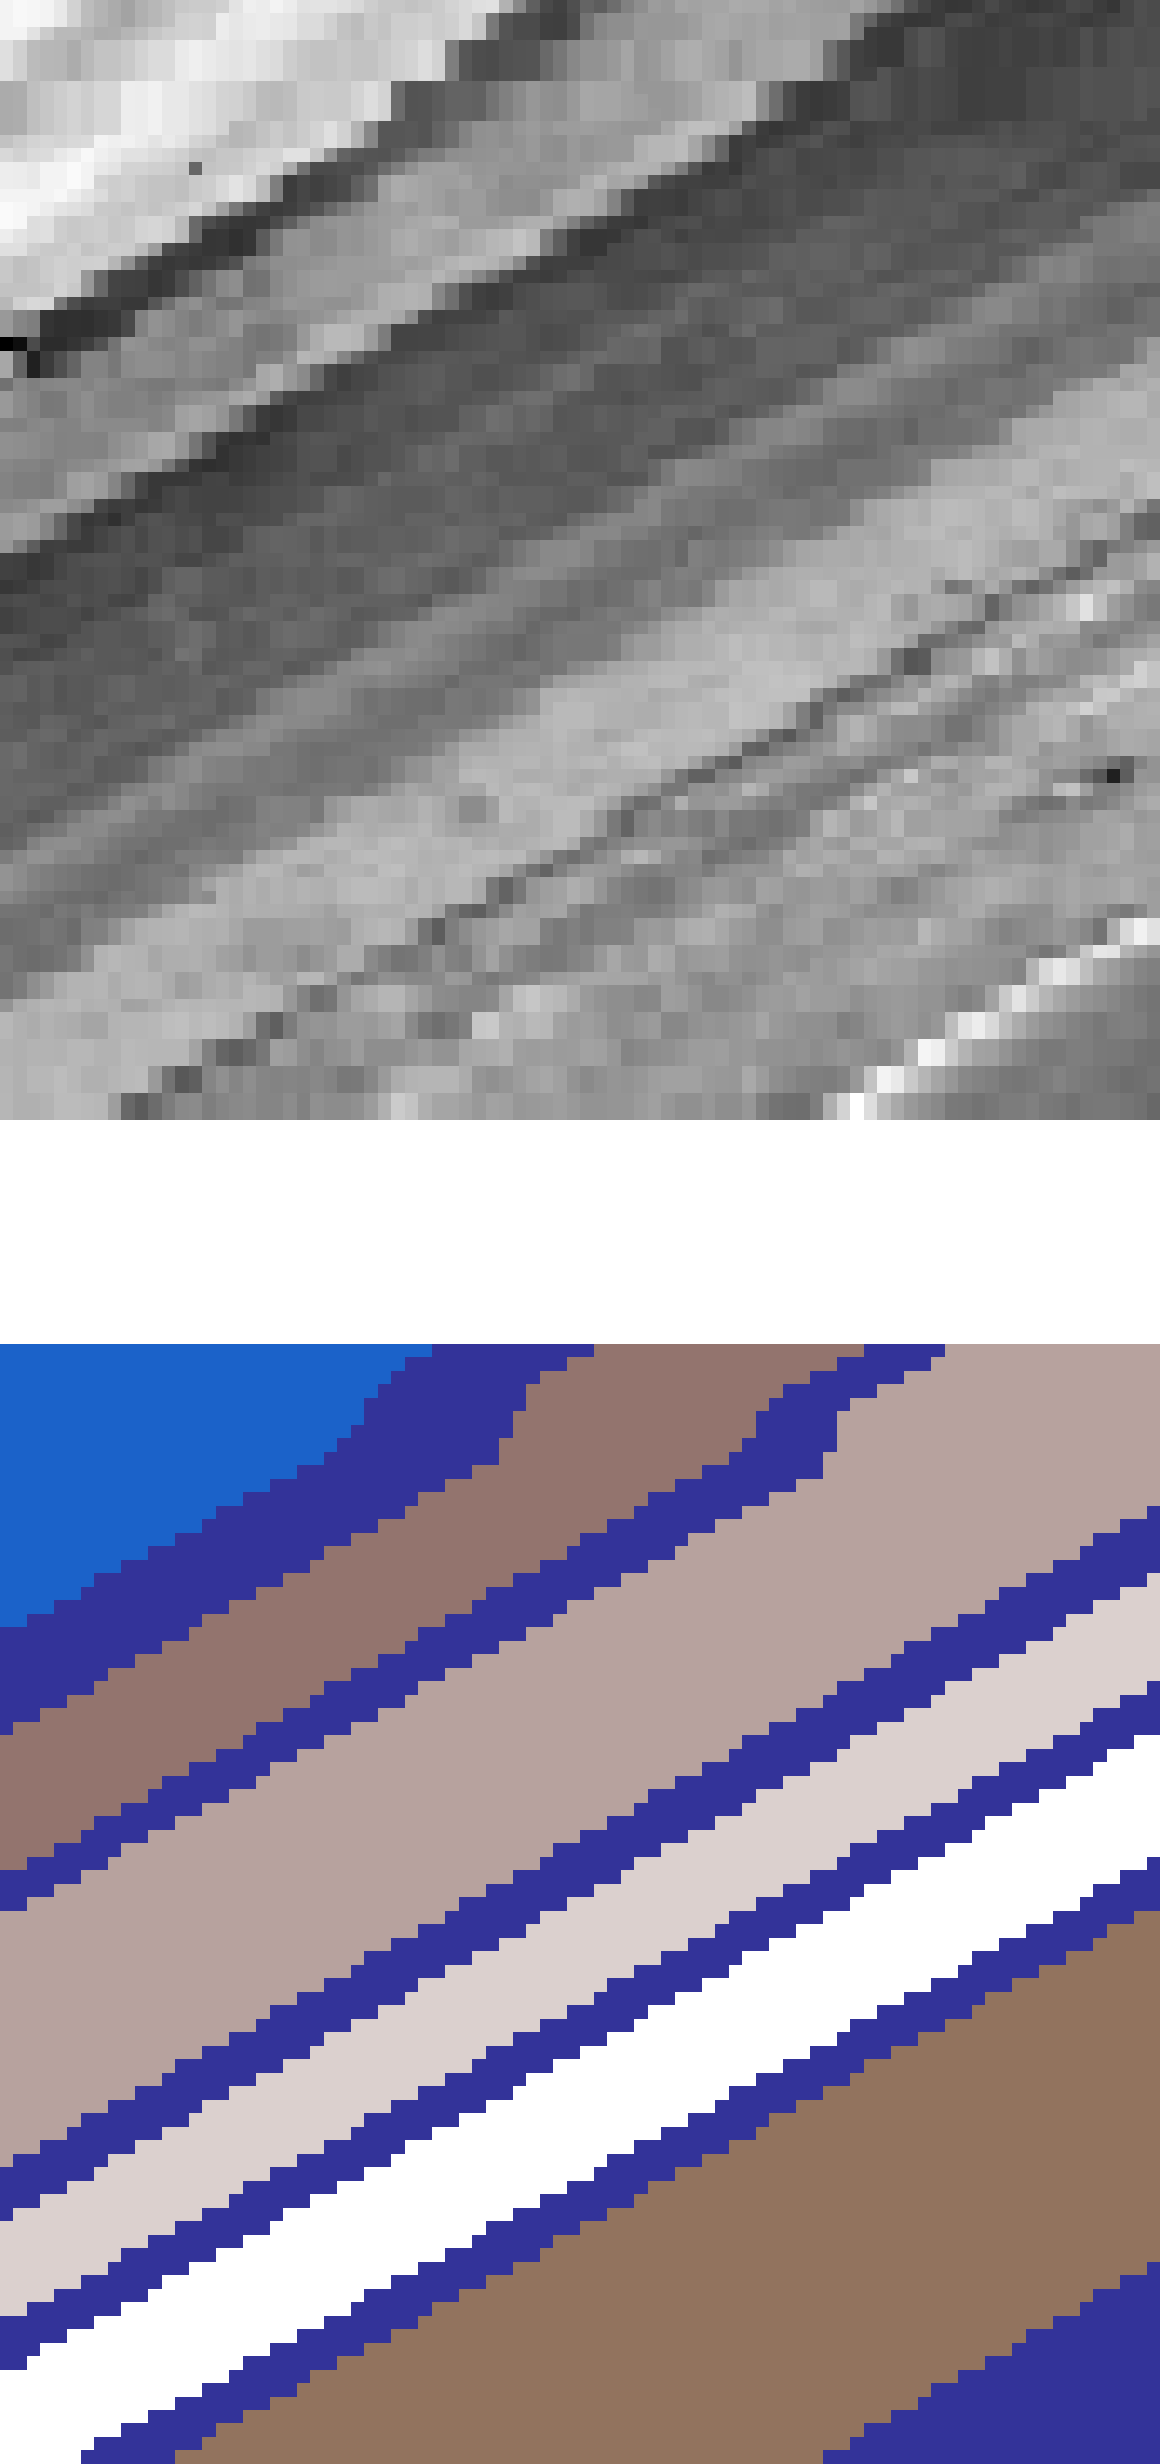
\includegraphics[height=1.9\linewidth]{../analysis/salinas_a}
		\subcaption{{\medbreak}}
		\label{fig:salinas_a}
	\end{subfigure}
	\begin{subfigure}{.24\textwidth}
		\centering
		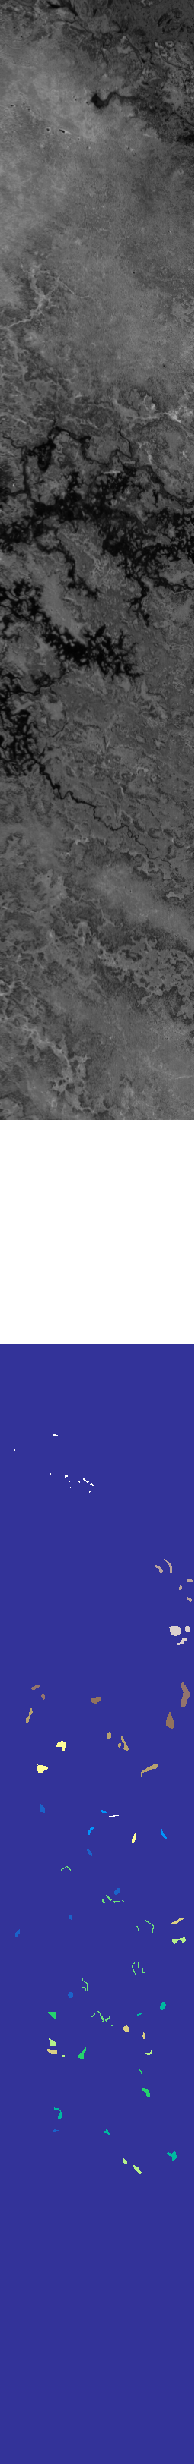
\includegraphics[height=1.9\linewidth]{../analysis/botswana}
		\subcaption{{\medbreak}}
		\label{fig:botswana}
	\end{subfigure}
	\begin{subfigure}{.24\textwidth}
		\centering
		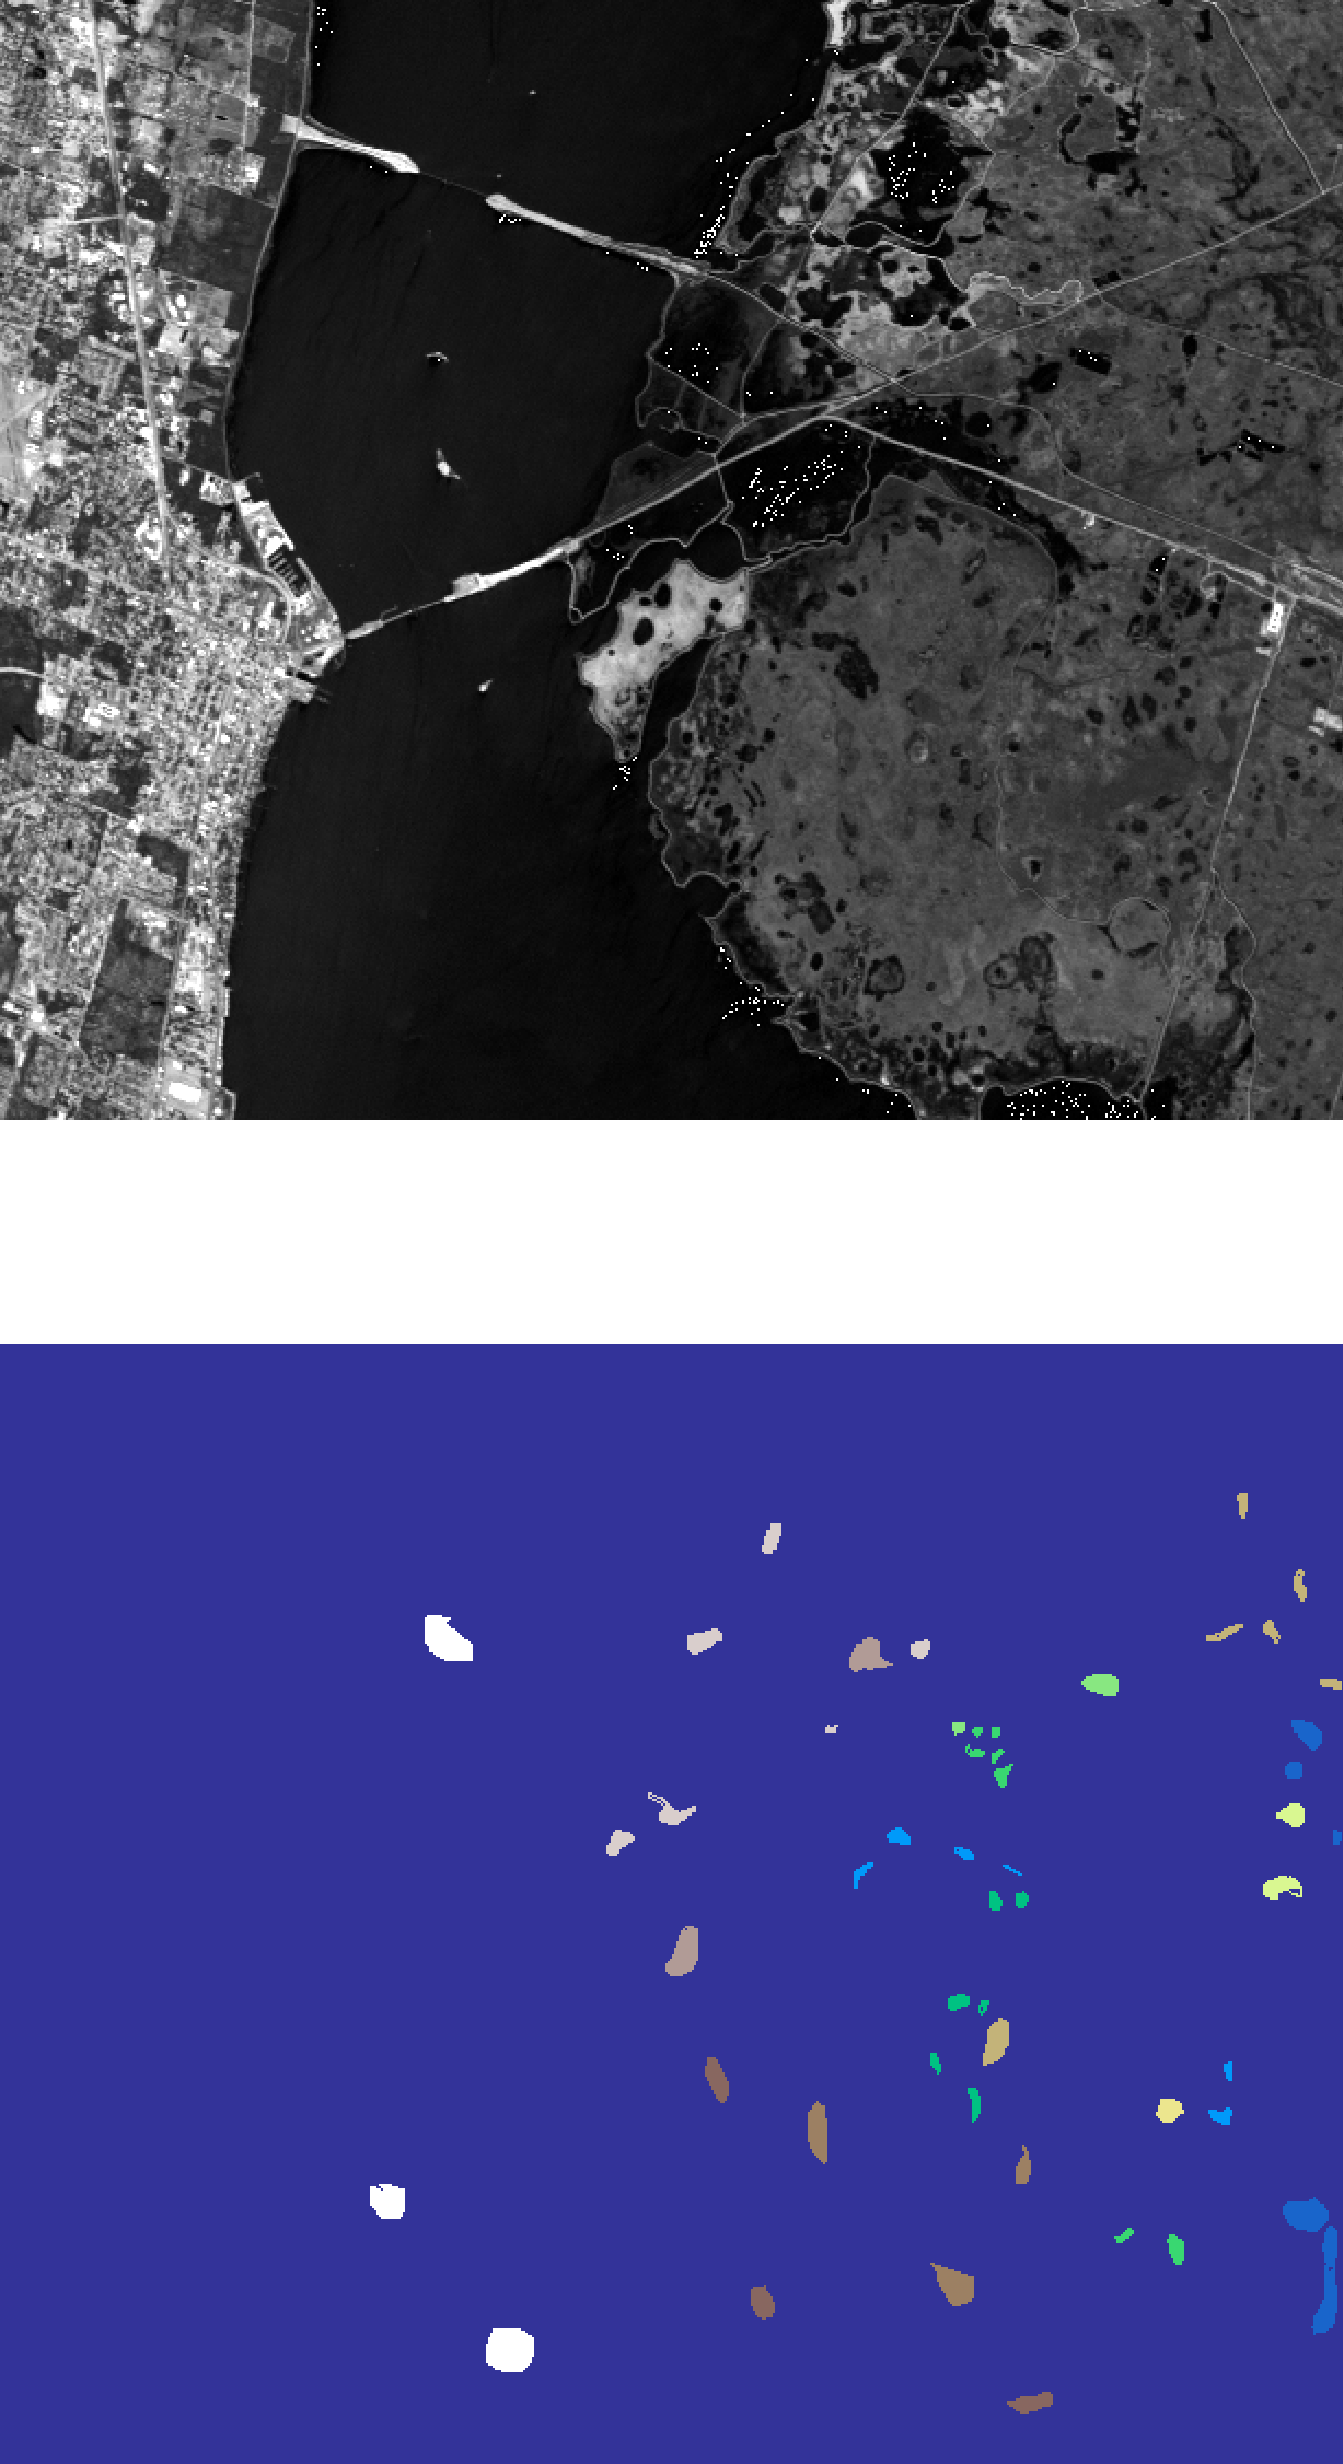
\includegraphics[height=1.9\linewidth]{../analysis/kennedy_space_center}
		\subcaption{{\medbreak}}
		\label{fig:kennedy_space_center}
	\end{subfigure}
	\caption{Gray scale visualization of a band (top row) and ground truth (bottom row) of
		each scene used in this study. (a) Indian Pines, (b) Pavia Centre, (c) Pavia
		University, (d) Salinas, (e) Salinas A, (f) botswana, (g) Kennedy Space Center}
	\label{fig:scenes}
\end{figure}

\subsection{Evaluation Metrics}
Most of the satellite-based LULC classification studies (nearly 80\%) employ
\textit{Overall Accuracy} (OA) and the \textit{Kappa Coefficient}
\cite{Gavade2019}. Although, some authors argue that both evaluation
metrics, even when used simultaneously, are insufficient to fully address the
area estimation and uncertainty information needs \cite{Olofsson2013,Pontius2011}.
Other metrics like User's Accuracy (or \textit{Precision}) and Producer's
Accuracy (or \textit{Recall}) are also common metrics to evaluate
per-class prediction power. These metrics consist of ratios employing the True
and False Positives (\textit{TP} and \textit{FP},
number of correctly/incorrectly classified observations of a given class) and
True and False Negatives  (\textit{TN} and \textit{FN},
number of correctly/incorrectly classified observations as not belonging to a
given class). These metrics are formulated as $Precision = \frac{TP}{TP+FP}$ and
$Recall = \frac{TP}{TP+FN}$. While metrics like OA and \textit{Kappa Coefficient} are
significantly affected by imbalanced class distributions,
\textit{F-Score} is less sensitive to data imbalance and a more
appropriate choice for performance evaluation \cite{Jeni2013}.

The datasets used present significantly high IRs (see Table
\ref{tab:datasets_description}). Therefore, it is especially important to attribute
equal importance to the predictive power of all classes, which does not happen
with OA and \textit{Kappa Coefficient}. In this study, we employ 3 evaluation
metrics: 1) \textit{G-mean}, since it is not affected by skewed class
distributions, 2) \textit{F-Score}, as it proved to be a more
appropriate metric for this problem when compared to other commonly used
metrics \cite{Jeni2013}, and 3) \textit{Overall Accuracy}, for discussion
purposes.

\begin{itemize}
	\item The \textit{G-mean} consists of the geometric mean of
	      $Specificity = \frac{TN}{TN + FP}$ and \textit{Sensitivity} (also known as \textit{Recall}). For multiclass problems, The
	      \textit{G-mean} is expressed as:

	      $$\textit{G-mean} = \sqrt{ \overline{Sensitivity} \times
			      \overline{Specificity}}$$

	\item \textit{F-score} is the harmonic mean of \textit{Precision} and
	      \textit{Recall}. The \textit{F-score} for the multi-class case can
	      be calculated using their average per class values \cite{He2009}:

	      $$\textit{F-score}=2\frac{\overline{Precision} \times \overline{Recall}}{\overline{Precision} +
			      \overline{Recall}}$$

	\item \textit{Overall Accuracy} is the number of correctly classified observations
	      divided by the total amount of observations. Having \( c \) as the label of the
	      various classes, \textit{Accuracy} is given by the following formula:

	      $$\textit{Accuracy} = \frac{ \sum\limits_{c}{ \text{TP}_{c} } }{
			      \sum\limits_{c}{ (\text{TP}_{c}  + \text{FP}_{c}) } } $$

\end{itemize}

\subsection{Machine Learning Algorithms}
The assess the quality of the K-SMOTE algorithm, five other oversampling
algorithms were used for benchmarking. ROS and SMOTE were chosen for their
simplicity and popularity. ADASYN and B-SMOTE were chosen for their popularity
as outperforming modifications of the SMOTE algorithm. G-SMOTE was chosen for
being a state-of-the-art oversampler and was found to outperform all of the
other benchmark oversamplers in a past study \cite{Douzas2019rs}. In
addition to the oversamplers mentioned, we present as the baseline method the
classification results without any oversampling method (NONE).

To assess the performance of each oversampler, we use the classifiers Logistic
Regression (LR) \cite{McCullagh1989}, K-Nearest Neighbors (KNN)
\cite{Cover1967}, Decision Tree (DT) \cite{Salzberg1994}, Gradient
Boosting Classifier (GBC) \cite{Friedman2001} and Random Forest (RF)
\cite{Liaw2002}. This choice was based on the classifiers' popularity
for LULC classification, learning type and training time
\cite{Maxwell2018,Gavade2019}.

\subsection{Experimental Procedure}
The procedure for the experiment reported in this study is similar to the one
proposed in \cite{Douzas2019rs}. We start by defining a parameter search
grid, where a list of possible values for each relevant hyperparameter in both
classifiers and oversamplers is stored. Based on this search grid, all possible
combinations of oversamplers, classifiers and parameters definitions are
formed. Finally, for each dataset we employ a $k$-fold
cross-validation strategy where $k=5$ to train each model
defined and save the averaged scores of each split.

Each combination of oversampler, classifier and parameters definition is fit 5
times (once for each fold) per dataset. Each time, an oversampler will use the
training set ($80\%$ of the dataset) to generate a set with
artificial data, which is appended to the original training set in order to
generate a training dataset with the exact same number of observations for each
class. The newly formed training dataset is used to train the classifier and
the test set ($20\%$ of the dataset, the remaining fold) is
used to evaluate the performance of the classifier. The evaluation scores are
then averaged over the 5 times the process is repeated. The range of
hyperparameters used are shown in table \ref{tab:grid}.

\begin{table}[H]
	\centering
	\begin{tabular}{lll}
		\toprule
		Classifier       & Hyperparameters      & Values                            \\
		\hline
		LR               & maximum iterations   & 10000                             \\
		KNN              & \# neighbors  & {3, 5}                            \\
		DT               & maximum depth        & {3, 6}                            \\
		GBC              & maximum depth        & {3, 6}                            \\
		                 & \# estimators & {50, 100}                         \\
		RF               & maximum depth        & {None, 3, 6}                      \\
		                 & \# estimators & {50, 100}                         \\
		\toprule
		Oversampler      &                      &                                   \\
		\hline
		K-SMOTE          & \# neighbors  & {3, 5}                            \\
		                 & \# clusters (as \% of number of observations)   & {0.1, 0.2, 0.4, 0.5, 0.6, 0.8, 0.9}      \\
		SMOTE            & \# neighbors  & {3, 5}                            \\
		BORDERLINE SMOTE & \# neighbors  & {3, 5}                            \\
		\bottomrule
	\end{tabular}
	\caption{\label{tab:grid}Hyperpameters grid.}
\end{table}

\subsection{Software Implementation}
The experiment was implemented using the Python programming language, using the
\href{https://scikit-learn.org/stable/}{Scikit-Learn} \cite{Pedregosa2011}, \href{https://imbalanced-learn.org/en/stable/}{Imbalanced-Learn}
\cite{JMLR:v18:16-365}, \href{https://geometric-smote.readthedocs.io/en/latest/?badge=latest}{Geometric-SMOTE}, \href{https://cluster-over-sampling.readthedocs.io/en/latest/?badge=latest}{Cluster-Over-Sampling} and
\href{https://research-learn.readthedocs.io/en/latest/?badge=latest}{Research-Learn} libraries. All functions, algorithms, experiments and
results are provided at the \href{https://github.com/joaopfonseca/publications/tree/master/remote-sensing-kmeans-
	smote}{GitHub repository of the project}.

\section{Results} \label{sec:results}

\pgfplotstabletypeset[
	begin table=\begin{longtable},
		end table=\end{longtable},  col sep=comma, header=true,
	columns={Classifier,Metric,NONE,ROS,SMOTE,B-SMOTE,K-SMOTE}, string type, every head row/.style={before row=\toprule, after row=\midrule\endhead},
	every last row/.style={after row=\bottomrule \caption{\label{tab:mean_sem_scores}
				Mean cross-validation scores of oversamplers.}}
]{../analysis/mean_sem_scores.csv}

\pgfplotstabletypeset[
	begin table=\begin{longtable},
		end table=\end{longtable},  col sep=comma, header=true,
	columns={Classifier,Metric,Difference}, string type, every head row/.style={before row=\toprule, after row=\midrule\endhead},
	every last row/.style={after row=\bottomrule \caption{\label{tab:mean_sem_perc_diff_scores}
				Results for percentage difference between K-SMOTE and SMOTE.}}
]{../analysis/mean_sem_perc_diff_scores.csv}

\pgfplotstabletypeset[
	begin table=\begin{longtable},
		end table=\end{longtable},  col sep=comma, header=true,
	columns={Classifier,Metric,NONE,ROS,SMOTE,B-SMOTE,K-SMOTE}, string type, every head row/.style={before row=\toprule, after row=\midrule\endhead},
	every last row/.style={after row=\bottomrule \caption{\label{tab:mean_sem_ranking}
				Results for mean ranking of oversamplers across datasets.}}
]{../analysis/mean_sem_ranking.csv}

\subsection{Statistical Analysis}

\pgfplotstabletypeset[
	begin table=\begin{longtable},
		end table=\end{longtable},  col sep=comma, header=true,
	columns={Classifier,Metric,p-value,Significance}, string type, every head row/.style={before row=\toprule, after row=\midrule\endhead},
	every last row/.style={after row=\bottomrule \caption{\label{tab:friedman_test}
				Results for Friedman test. Statistical significance is tested at a level of
				$\alpha = 0.05$.}}
]{../analysis/friedman_test.csv}

\pgfplotstabletypeset[
	begin table=\begin{longtable},
		end table=\end{longtable},  col sep=comma, header=true,
	columns={Classifier,Metric,NONE,ROS,SMOTE,B-SMOTE}, string type, every head row/.style={before row=\toprule, after row=\midrule\endhead},
	every last row/.style={after row=\bottomrule \caption{\label{tab:holms_test}
				Adjusted p-values using the Holm's method.}}
]{../analysis/holms_test.csv}

\section{Conclusion} \label{sec:conclusion}

\bibliography{references}
\bibliographystyle{apalike}

\end{document}
